\section{Experiments}
\subsection{Datasets and Metrics}
Our experiments were conducted on a subset of ImageNet-1K \cite{deng2009imagenet}. Specifically, we randomly sample only 4,096 images ($<0.32 \%$) from the training set for training and 1,000 images from the validation set for testing.

We employ a comprehensive set of Image Quality Assessment (IQA) metrics. For full-reference IQA, we use the Peak Signal-to-Noise Ratio (PSNR), Structural Similarity Index Measure (SSIM), and LPIPS \cite{zhang2018unreasonable}. 
For no-reference IQA, we utilize the Natural Image Quality Evaluator (NIQE) \cite{mittal2012making} and MANIQA \cite{yang2022maniqa}. 
Furthermore, to measure the eavesdropping information accuracy, we assess the inversion image top-1 classification accuracy (\textbf{Acc}) with the GT label of the original image, using ResNet-50 \cite{he2016deep}.
To assess private information leakage, we propose two novel metrics evaluated by Large Vision-Language Models (LVLMs): LVLM-Consistency (\textbf{LVLM-C}) and LVLM-Privacy-Leakage (\textbf{LVLM-PL}).
As shown in Fig. \ref{fig-lvlm}, the LVLM acts as an \textit{Image Description Expert}, generating textual descriptions for both the original and inversion images.
These descriptions are compared by an \textit{Image Leak Inspector} to determine whether they depict the same primary object (LVLM-C) and to compute their semantic similarity via BERTScore \cite{zhang2019bertscore} (LVLM-PL).
Higher LVLM-C and LVLM-PL values indicate that the attacker can extract more detailed private information from the inversion image.
In our implementation, we utilize \textit{gpt-4o-mini} as the LVLM. 
See supplementary materials for the detailed calculation process and an ablation study with other LVLM.
\begin{table*}[t]
\setlength{\tabcolsep}{1.4mm}
\caption{The performance comparison among different FIA methods. Bold indicates the best result of all methods.}
\label{table-compare}
\renewcommand\arraystretch{0.7}
\centering
\begin{tabular}{ccccccccccc}
\toprule
Model & Layer & Method & PSNR $\uparrow$& SSIM $\uparrow$& LPIPS $\downarrow$ & Acc $\uparrow$& LVLM-C $\uparrow$& LVLM-PL $\uparrow$& NIQE $\downarrow$ & MANIQA $\uparrow$\\
  \midrule
 \multirow{6}{*}{AlexNet} & \multirow{6}{*}{F-10} & M\&V & 13.55 & 0.500 & 0.730 & 0.0 & 1.2&0.860 & 5.853 & 0.4303 \\
 & & DIP &15.45 &0.422 &0.585  &16.1 &10.6&0.880 & 5.988 &0.2763 \\
 & & AR & 18.65 & 0.508 & 0.574 & 4.1 & 4.8 & 0.880 & 5.874 &0.3258 \\
  & & SG-DIP & 11.07&0.257 &0.778  & 1.2&3.6 & 0.865 &\textbf{5.603} &0.2950 \\
  & & FIA-Align &20.46 & \textbf{0.607}  &0.620 & 5.7&9.3& 0.883&10.927 &0.2959  \\
 & & \cellcolor{myhighlight}FIA-Flow & \cellcolor{myhighlight}\textbf{20.64}& \cellcolor{myhighlight}0.603&\cellcolor{myhighlight}\textbf{0.405}  &\cellcolor{myhighlight}\textbf{28.8}& \cellcolor{myhighlight}\textbf{16.6}& \cellcolor{myhighlight}\textbf{0.900}& \cellcolor{myhighlight}6.243&\cellcolor{myhighlight}\textbf{0.4956}  \\
 \midrule
\multirow{10}{*}{ResNet-50} & \multirow{5}{*}{L1-2} & M\&V & 13.83 & 0.603 & 0.593 & 13.4 &17.5  &0.903  & 5.392 & 0.4938\\
 & & DIP & 25.73 & 0.706 & 0.236 & 61.0 &  39.9&0.905 & 5.504 & 0.4565 \\
  & & SG-DIP & 27.90&0.754 &0.193  & 65.2& 65.3 &0.922 &5.301 &0.4928 \\
  & & FIA-Align & 29.86 & 0.810&0.157  & 64.3& 70.0&0.923 & 5.136 & 0.5622 \\
 & & \cellcolor{myhighlight}FIA-Flow &\cellcolor{myhighlight}\textbf{30.01} &\cellcolor{myhighlight}\textbf{0.814} &\cellcolor{myhighlight}\textbf{0.100}  &\cellcolor{myhighlight}\textbf{71.3}&\cellcolor{myhighlight}\textbf{70.1} & \cellcolor{myhighlight}\textbf{0.929}& \cellcolor{myhighlight}\textbf{4.408}&\cellcolor{myhighlight}\textbf{0.6131}  \\
\cmidrule{2-11}
 & \multirow{5}{*}{L4-2} & M\&V & 13.55 & 0.504 & 0.851 & 0.0&3.0 &  0.860 & 7.577 & 0.4359\\
 & & DIP & 13.60 & 0.453 & 0.711 &27.3 & 9.4 &0.881 &7.152 & 0.2592 \\
  & & SG-DIP &11.59 &0.309 &0.777  & 8.1&5.0 &0.872&5.603 &0.3189 \\
   & & FIA-Align & \textbf{20.36} & \textbf{0.603} & 0.643  &4.4&6.3&0.878 & 11.309 &0.2969\\
 & & \cellcolor{myhighlight}FIA-Flow & \cellcolor{myhighlight}20.31 & \cellcolor{myhighlight}0.584 & \cellcolor{myhighlight}\textbf{0.397} & \cellcolor{myhighlight}\textbf{36.8} & \cellcolor{myhighlight}\textbf{18.0} & \cellcolor{myhighlight}\textbf{0.902} & \cellcolor{myhighlight}\textbf{5.098} & \cellcolor{myhighlight}\textbf{0.5628} \\
 \midrule
 \multirow{5}{*}{Swin-B}& \multirow{5}{*}{F3-2} & M\&V &14.34 &0.628 &0.541  & 38.1& 38.4& 0.913&6.105 & 0.4465\\
 & & DIP & 21.03&0.735 &0.313  & 61.7& 54.5&0.920 &5.486 &0.4492 \\
  & & SG-DIP&25.15 &\textbf{0.872} &0.191  & 68.5&62.3 & 0.913&5.520 &0.5362 \\
  & & FIA-Align & 26.64& 0.771&0.260  & 53.6& 51.5&0.919 &6.236 &0.4725 \\
   & & \cellcolor{myhighlight}FIA-Flow &
    \cellcolor{myhighlight}\textbf{27.29} &
    \cellcolor{myhighlight}0.780 &
    \cellcolor{myhighlight}\textbf{0.159} &
    \cellcolor{myhighlight}\textbf{70.6} &
    \cellcolor{myhighlight}\textbf{63.2} &
    \cellcolor{myhighlight}\textbf{0.925} &
    \cellcolor{myhighlight}\textbf{4.840} &
    \cellcolor{myhighlight}\textbf{0.5777} \\
\midrule
  \multirow{5}{*}{YOLO11n}& \multirow{5}{*}{M-8} & M\&V &7.59 &0.239 &0.890 &0.3 & 1.2& 0.863&6.715 & 0.4702\\
 & & DIP & 14.09&0.521 &0.572 & 14.6& 18.2&0.897 & 6.796&0.4168 \\
  & & SG-DIP& 14.04&0.518 &0.582 & 12.1& 18.1& \textbf{0.899}&6.696 &0.4124 \\
  & & FIA-Align &20.56 &\textbf{0.612} &0.627 & 4.1& 7.1&0.880 &11.056 & 0.2958\\
   & & \cellcolor{myhighlight}FIA-Flow &
    \cellcolor{myhighlight}\textbf{20.90} &
    \cellcolor{myhighlight}0.608&
    \cellcolor{myhighlight}\textbf{0.437} &
    \cellcolor{myhighlight}\textbf{23.6} &
    \cellcolor{myhighlight}\textbf{23.9} &
    \cellcolor{myhighlight}\textbf{0.899} &
    \cellcolor{myhighlight}\textbf{6.528} &
    \cellcolor{myhighlight}\textbf{0.4968} \\
    \midrule
     \multirow{5}{*}{DINOv2-B}& \multirow{5}{*}{B-11} & M\&V & 13.53&0.477 &0.868 &0.1 &0.7 &0.855 &13.533 &0.3324 \\
 & & DIP & 13.45& 0.493&0.833 &1.3 & 4.9& 0.868& 8.497 &0.3316\\
  & & SG-DIP&12.42 &0.345&0.741 & 17.7 &28.3 & 0.905&5.838 &0.3662 \\
  & & FIA-Align &19.92 &0.619 &0.609 &9.2 & 16.7& 0.890&10.340 &0.2709 \\
   & & \cellcolor{myhighlight}FIA-Flow &
    \cellcolor{myhighlight}\textbf{20.13} &
    \cellcolor{myhighlight} \textbf{0.621}&
    \cellcolor{myhighlight}\textbf{0.411} &
    \cellcolor{myhighlight}\textbf{42.8} &
    \cellcolor{myhighlight}\textbf{30.4} &
    \cellcolor{myhighlight}\textbf{0.909} &
    \cellcolor{myhighlight}\textbf{6.304} &
    \cellcolor{myhighlight}\textbf{0.5079} \\

\bottomrule
\end{tabular}
\end{table*}

\subsection{Implementation Details}
We selected \textit{features.10} (F-10) of AlexNet \cite{krizhevsky2017imagenet}, \textit{layer1.2} (L1-2) and \textit{layer4.2} (L4-2) of ResNet-50 \cite{he2016deep}, \textit{features.3.0.mlp.2} (F3-2) of Swin Transformer (Swin-B) \cite{liu2021swin}, \textit{model.8} (M-8) of YOLO11n \cite{yolo11_ultralytics}, and \textit{blocks.11} (B-11) of DINOv2-B \cite{oquab2023dinov2} as the victim layers and models for FIA.
The DIFM is initialized with the pre-trained weights of Stable Diffusion 2.1 \cite{rombach2022high}. 
To adapt it for the FIA task, we freeze the U-Net in the DIFM and integrate a Low-Rank Adaptation (LoRA) \cite{lora} model with a rank of $r=4$.
For both stages, we set the batch size to $8$ and the learning rate to $0.0001$, with each stage trained for $64,000$ iterations.
All experiments were conducted on NVIDIA A100 GPUs.

\begin{figure*}[t]
    \centering
    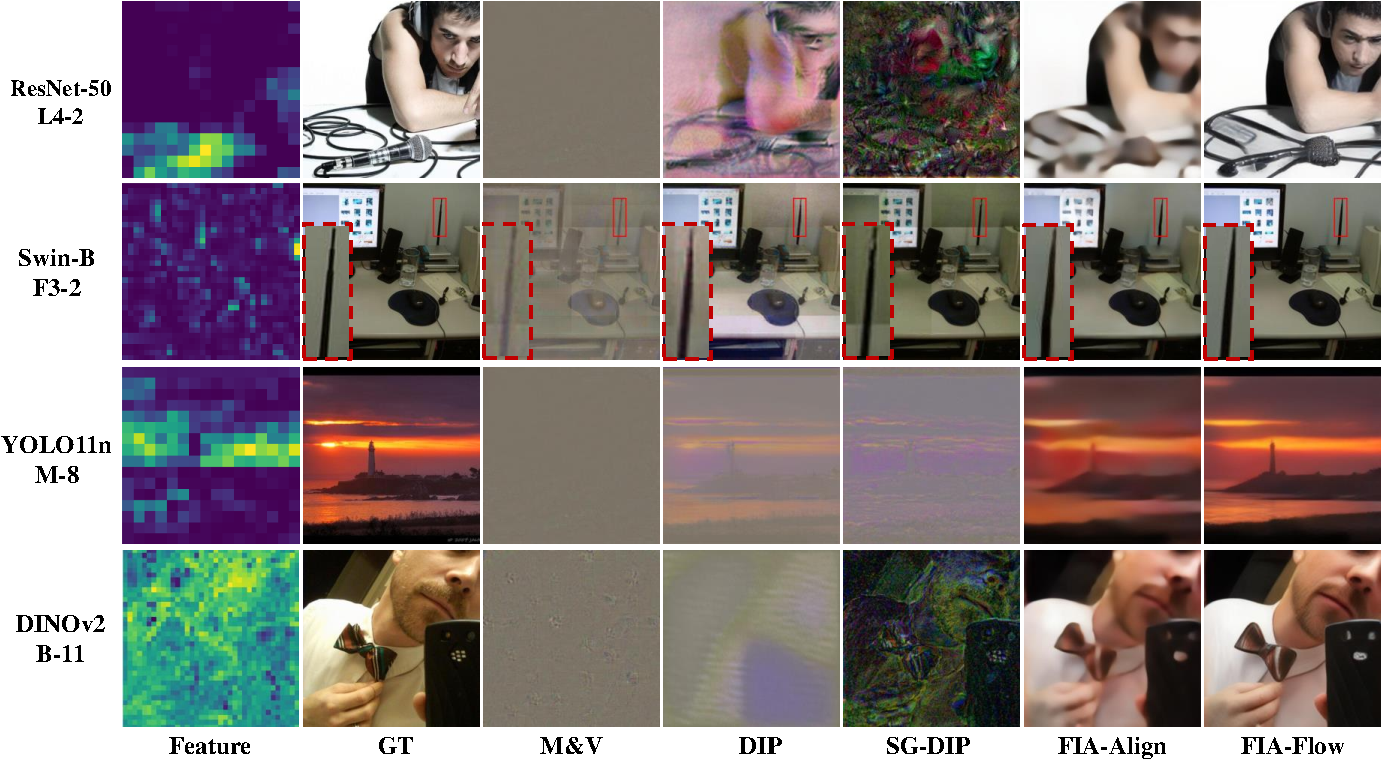
\includegraphics[width=0.9\linewidth]{img/fig-compare-2.pdf}
    \caption{Visualization comparison of different FIA methods on various models. 
    }
    \label{fig-compare}
\end{figure*}
\begin{figure}[t]
    \centering
    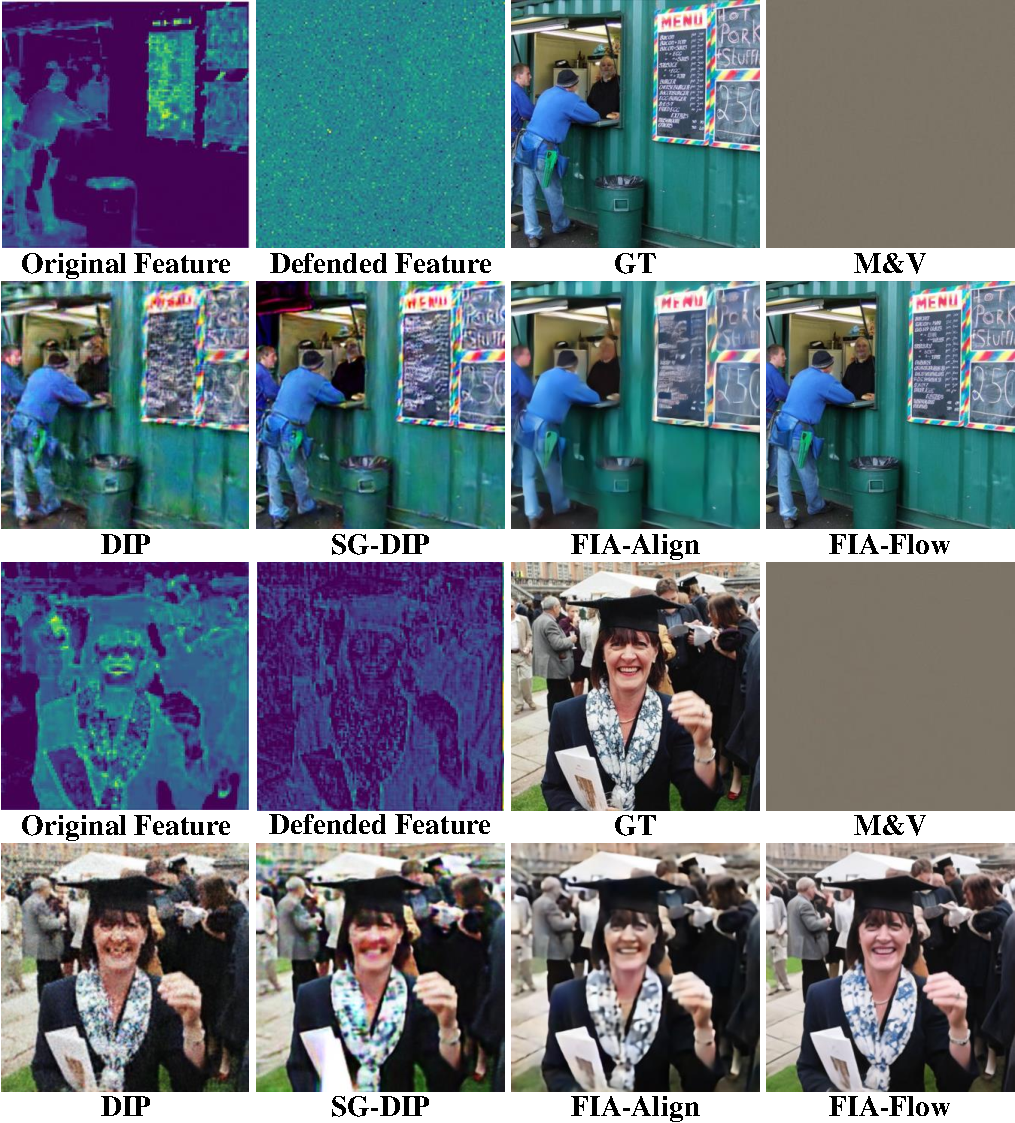
\includegraphics[width=0.9\linewidth]{img/fig-defend-1112.pdf}
    \caption{Visualization comparison on different defense mechanisms. Top row: visualizations under the Noise+NoPeek defense \cite{titcombe2021practical}. Bottom row: visualizations under the DISCO defense \cite{singh2021disco}.}
    \label{fig-defend}
\end{figure}


\subsection{Main results}
We compare the proposed FIA-Flow with state-of-the-art FIA methods, including M\&V \cite{mahendran2015understanding}, Deep Image Prior (DIP) \cite{dmitry2020deep}, Adversarially Robust (AR) \cite{rojas2022inverting}, Self-Guided DIP (SG-DIP) \cite{liang2025analysis}. 
Additionally, we compared against a baseline FIA-Align that solely employs LFSAM for feature space alignment, followed by VAE decoding.


\paragraph{Quantitative Results}
Table \ref{table-compare} shows the results of different FIA methods for various victim models and layers.
For AlexNet, FIA-Flow achieves an Acc of 28.8\%, showing a significant advantage over other methods.
For ResNet-50, when dealing with information-rich shallow features (L1-2), FIA-Flow can achieve an outstanding Acc of \textbf{71.3\%}.
This performance remains robust even when dealing with deep features from the L4-2 layer, which typically suffer from substantial information loss. 
While other methods experience a dramatic degradation in image quality, leading to significant drops in both Acc and LVLM-based evaluations, FIA-Flow maintains an Acc of 36.8\% and an LVLM-PL of 0.902. 
Furthermore, experiments on the Swin Transformer model (Swin-B), object detection model (YOLO11n), and foundation model (DINOv2-B) confirm the superiority of FIA-Flow, highlighting its broad applicability and effectiveness across diverse model architectures.

Benefiting from the alignment-refinement strategy, FIA-Flow not only achieves a higher inversion quality on IQA metrics but also exhibits substantially better semantic preservation, as validated by Acc and LVLM-based metrics. 
This proves that FIA-Flow constitutes a more effective and practical privacy threat.

\paragraph{Qualitative Results}
As shown in Fig. \ref{fig-compare}, our FIA-Flow outperforms other methods on both ResNet-50, Swin-B, YOLO11n, and DINOv2. 
While other methods fail or produce blurry results, FIA-Flow can invert images with exceptional clarity, accurately capturing fine details like the face, wireless router, and lighthouse. 
This visually confirms its state-of-the-art performance and robustness across diverse architectures. 
More visual results are available in the Supplementary Materials.

\paragraph{Robustness Evaluation Under Defenses}
To verify the robustness of FIA-Flow under different defense mechanisms, we evaluate all methods against two representative defenses: Noise+NoPeek \cite{titcombe2021practical} and DISCO \cite{singh2021disco}, as shown in Table \ref{ab-defend} and Fig. \ref{fig-defend}.
Under the Noise+NoPeek defense, where Laplacian noise is injected into intermediate features and a NoPeek strategy \cite{vepakomma2020nopeek} is employed to restrict information leakage, FIA-Flow still outperforms other methods. 
Similarly, under the DISCO defense, which suppresses intermediate features, FIA-Flow remains effective, recovering the original image with minimal samples.
This demonstrates that FIA-Flow can effectively bypass defense mechanisms and extract sensitive information, even in a black-box setting, without access to the defense's implementation details and model parameters.

\begin{table}[t]
\caption{Robustness comparison under different defense mechanisms of Split DNNs on the L1–2 layer of ResNet-50.}
\setlength{\tabcolsep}{0.6mm}
\centering
\label{ab-defend}
\renewcommand\arraystretch{0.8}
\begin{tabular}{cccccc}
\toprule
Defense& Methods& PSNR$\uparrow$& Acc$\uparrow$& LVLM-C$\uparrow$& LVLM-PL$\uparrow$\\
\midrule
 \multirow{5}{*}{\shortstack{Noise\\+\\ NoPeek\\ \cite{titcombe2021practical}}}& M\&V&13.56&0.0 & 2.1&0.861\\
  &  DIP&21.87 &26.9& 41.5&0.921 \\
   & SG-DIP&21.69&53.3&49.1&0.919\\
 & FIA-Align&26.05 &38.3 & 45.8&0.911\\
 & \cellcolor{myhighlight}FIA-Flow & \cellcolor{myhighlight}\textbf{27.70} & \cellcolor{myhighlight}\textbf{62.2} & \cellcolor{myhighlight}\textbf{55.0} & \cellcolor{myhighlight}\textbf{0.922} \\
   \midrule
  \multirow{5}{*}{\shortstack{DISCO\\ \cite{singh2021disco}}}&  M\&V
&13.57&0.1&1.0&0.860\\
  & DIP&
\textbf{27.10}&35.9&39.6&0.914\\
  & SG-DIP
& 26.02&43.7&39.8 &0.910\\
 & FIA-Align&
26.49 &37.4 &38.7 &0.913\\
 & \cellcolor{myhighlight}FIA-Flow & \cellcolor{myhighlight}26.75 & \cellcolor{myhighlight}\textbf{59.0} & \cellcolor{myhighlight}\textbf{44.8} & \cellcolor{myhighlight}\textbf{0.916} \\
 \bottomrule
\end{tabular}
\end{table}



\paragraph{Generalization Evaluation Across Diverse Datasets}
We evaluate on the MS COCO-2017 dataset \cite{lin2014microsoft} to demonstrate the generalization capability of FIA-Flow (See Table~\ref{table-coco}). 
To quantify privacy leakage beyond standard IQA, we introduce the \textbf{Object Reconstruction Rate (ORR)}, which measures the consistency between the outputs of a pre-trained detector (Faster R-CNN \cite{ren2016faster}) on the original and inverted images.
Trained only on ImageNet and without fine-tuning on COCO,  FIA-Flow achieves state-of-the-art performance compared to methods that require sample-specific optimization on target features.
This cross-dataset generalization is mainly attributed to the alignment–refinement design of FIA-Flow, which learns a dataset-agnostic mapping from task features to the VAE latent space.
High ORR obtained by FIA-Flow indicates that the inverted images retain task-relevant semantics for downstream models, revealing a stronger privacy risk than IQA metrics alone capture.
The definition of ORR and the complete results are shown in the Supplementary Materials. 
\begin{table}[t]
\setlength{\tabcolsep}{1.0mm}
\renewcommand\arraystretch{0.8}
\caption{The performance comparison with different FIA methods on the COCO dataset. Bold indicates the best result of all methods.}
\centering
\label{table-coco}
\begin{tabular}{ccccc}
\toprule
 Method & LPIPS $\downarrow$ &MANIQA $\uparrow$ & $\text{ORR}_{0.5}$ $\uparrow$& $\text{ORR}_{0.75}$ $\uparrow$\\
  \midrule
 M\&V &0.700&0.5191&3.30&2.20\\
  DIP &0.332 
&0.4464&44.94&33.40\\
   SG-DIP &0.284
&0.4834&50.41&39.75\\
   FIA-Align & 0.195
&0.5981&56.02&45.84\\
  \cellcolor{myhighlight}FIA-Flow &\cellcolor{myhighlight}\textbf{0.115}&\cellcolor{myhighlight}\textbf{0.6626}&\cellcolor{myhighlight}\textbf{69.00}&\cellcolor{myhighlight}\textbf{59.33}\\
\bottomrule
\end{tabular}
\end{table}


\subsection{Ablation Studies}
We report the main ablation results on attack-layer robustness, data efficiency, and the diffusion sampling methods and steps in the main paper. 
Additional ablations and complete results are shown in the Supplementary Materials.
\paragraph{Results on Different Training Numbers}
To test data efficiency, we trained on the ResNet-50 L4-2 layer using datasets ranging from 4,096 (0.32\%) down to just \textbf{128 (0.01\%)} samples, shown in Table \ref{table-number} and Fig.~\ref{fig-duibi}(a). 
Using only 128 samples (0.01\%), FIA-Flow not only achieves a high Acc of 27.7\% but also outperforms other methods.
The data efficiency can be attributed to LFSAM, which enforces structural alignment with the latent space through feature rearrangement that matches its dimensionality and hierarchical aggregation that reduces the mapping complexity and sample requirements.
\paragraph{Results on Different Layers}
We evaluate FIA-Flow at various depths of ResNet-50, shown in Table \ref{table-layer} and Fig. \ref{fig-duibi}(b). 
While performance degrades in deeper layers, FIA-Flow consistently outperforms other methods across all victim layers.
Notably, its performance on the deep L3-2 layer (\textbf{69.8\%} Acc) exceeds SG-DIP's 65.2\% on the shallow L1-2 layer.
Despite the loss of spatial detail in deeper layers, FIA-Flow effectively uses high-level semantic information for accurate reconstruction.
This capability underscores a serious privacy concern: FIA-Flow can recover visually detailed and semantically meaningful images from abstract representations.

\begin{figure}[t]
    \centering
    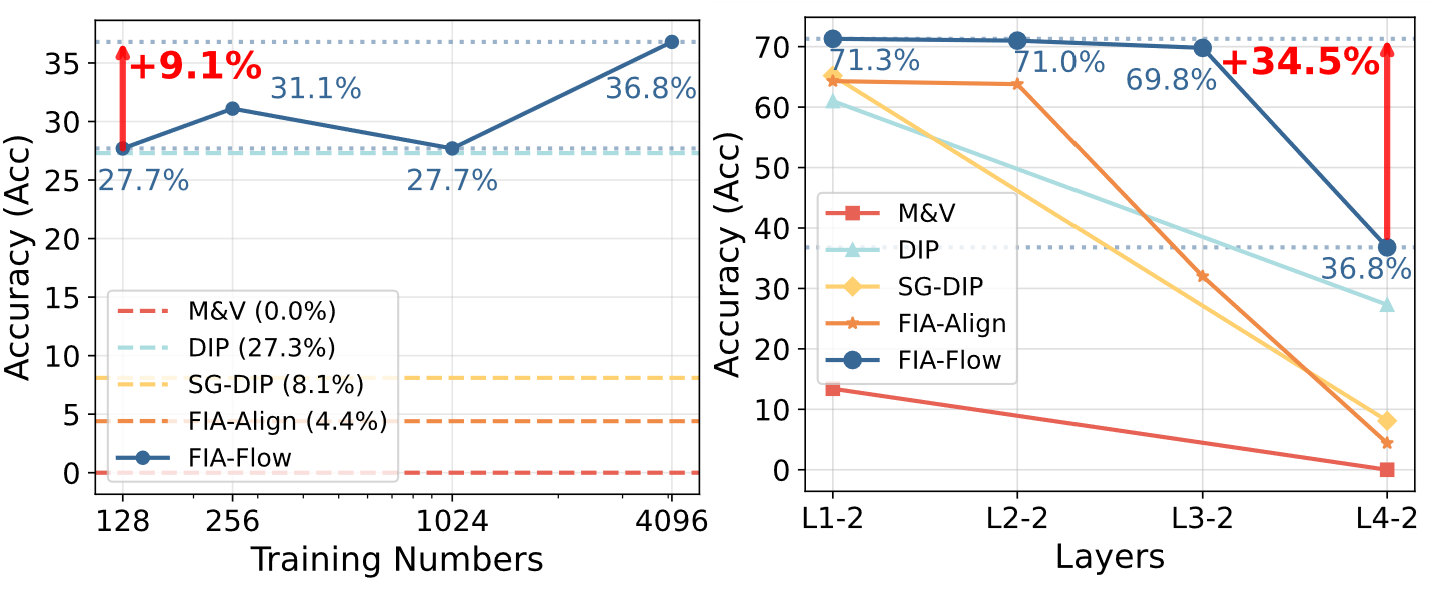
\includegraphics[width=\linewidth]{img/fig-ab-1113.pdf}
    \caption{(a) Left: Performance comparison on the L4-2 layer with different training numbers of FIA-Flow. (b) Right: Performance comparison at different layers.}
    \label{fig-duibi}
\end{figure}

\begin{table}[t]
\caption{The performance comparison of FIA-Flow with different training numbers on L4-2 of ResNet-50.}
\centering
\label{table-number}
\setlength{\tabcolsep}{1.0mm}
\begin{tabular}{ccccc}
\toprule
Number& PSNR $\uparrow$& Acc $\uparrow$& LVLM-C $\uparrow$& LVLM-PL $\uparrow$\\
\midrule
 \multirow{1}{*}{4,096(0.32\%)}  &20.31  &36.8&18.0 &0.902 \\
 \multirow{1}{*}{1024(0.08\%)} & 20.04 & 27.7&14.5 &0.898 \\
 \multirow{1}{*}{256(0.02\%)}  & 19.45 & 31.1& 12.8&0.900 \\
 \multirow{1}{*}{128(0.01\%)}  & 19.01 & 27.7&12.5 &0.898 \\
\bottomrule
\end{tabular}
\end{table}


\begin{table}[t]
\caption{The performance comparison of FIA-Flow across different victim layers of ResNet-50.}
\renewcommand\arraystretch{0.96}
\centering
\label{table-layer}
\begin{tabular}{ccccc}
\toprule
 Layer & PSNR $\uparrow$& Acc $\uparrow$& LVLM-C $\uparrow$& LVLM-PL $\uparrow$\\
  \midrule
 \multirow{1}{*}{L1-2} & 30.01 &71.3 &70.1 &0.929\\
  \multirow{1}{*}{L2-2} & 29.65 & 71.0 &69.8 &0.928\\
   \multirow{1}{*}{L3-2} & 26.29 & 69.8 &63.4 &0.913\\
  \multirow{1}{*}{L4-2} & 20.31  &36.8&18.0 &0.902 \\
 \bottomrule
\end{tabular}
\end{table}

\begin{table}[t]
\caption{The performance comparison of FIA-Flow with different sampling methods and steps on L4-2 of ResNet-50.}
\setlength{\tabcolsep}{1.0mm}
\renewcommand\arraystretch{0.7}
\centering
\label{table-step}
\begin{tabular}{cccccc}
\toprule
 Methods& Steps & PSNR$\uparrow$& Acc$\uparrow$& LVLM-C$\uparrow$& LVLM-PL$\uparrow$\\
\midrule
 \multirow{3}{*}{DDPM} & 10 &20.09 & 4.1& 5.8 &0.878 \\
  &  50 & 19.97&4.9 & 4.2& 0.876 \\
   & 200 &19.95 &4.5 & 4.8 &0.877\\
   \midrule
  \multirow{3}{*}{DIFM} &  1 &\textbf{20.31} &36.8 &18.0 &0.902 \\
  & 5 &19.61 &\textbf{38.2} &37.3 &\textbf{0.914} \\
  & 10 & 19.21&36.9 &\textbf{38.3} &\textbf{0.914} \\
\bottomrule
\end{tabular}
\end{table}





\paragraph{Results on Different Sampling Methods and Steps}
The performance gap between diffusion probabilistic model (DDPM) \cite{ho2020denoising} and DIFM reflects not only efficiency but also methodological suitability for FIA.
The iterative ``add-noise, then-denoise'' paradigm of DDPM is an indirect and stochastic process designed for diverse sampling, making it difficult for the high-fidelity reconstruction of a specific input. 
In contrast, FIA-Flow adopts a deterministic alignment-refinement paradigm, enabling efficient, high-fidelity inversion.
As shown in Table \ref{table-step}, one-step DIFM is highly effective. 
Increasing sampling steps slightly decreases PSNR but improves Acc and LVLM-based scores, suggesting increased privacy exposure.

